\section{Acceptance/Rejection \\Method}
The Acceptance-Rejection Method is a way to draw random deviates from a density function, $p(x)$. The steps are the following:
\begin{enumerate}
    \item Choose a function $f(x) > p(x)$ for all $x$ and make sure it is an integrable function.
    \item Calculate the total area of $f(x)$ and draw a uniform random deviate,$y \in [0,A_T]$.
    \item Evaluate the inverse function $f^{-1}(x)=F(y)$ to find $x_0$.
    \item Draw a second uniform random deviate, $f_1 \in[0,f(x_0)]$.
    \item Evaluate the density function $p(x_0)=p_1$ and if $f_1\leq p_1$, accept $x_0$ as a random deviate of the density function $p(x)$. Otherwise, reject the value and start process again.
\end{enumerate}

The set of accepted $x_0$ will map the density function $p(x)$. 


For this problem, we define p(x) to be 


% Use the Acceptance-Rejection Method to
% draw random deviates from a probability distribution shaped like the first half-cycle of a sine
% function (properly normalized) on the interval $[0,\pi]$.I would like you to use two different
% functions for $f(x)$:
% \begin{enumerate}
%     \item a constant $f(x)$ for the full interval
%     \item any other non-constant function of your choice.
% \end{enumerate}

% In each case you should compare the sine wave to a histogram your random deviates to show
% that you have faithfully sampled from the distribution. Finally, for each case show that the
% inefficiency factor (the number of trials you have to make divided by the number of good deviates
% that you get) is equal to the area under $f(x)$ on the interval $[0,\pi]$. Note that the function that
% you choose must have an efficiency factor that is smaller than that of the constant function.


\begin{table}
    \centering
    \begin{tabular}{lcc}
\toprule
{} &  Ineficiency Factor &  Total Area \\
\midrule
Constant  &                1.8776 &       1.8850 \\
Quadratic &                1.1912 &       1.1906 \\
\bottomrule
\end{tabular}

    \caption{Table that shows the total area and the inefficiency factor.}
    \label{tab:accRej}
\end{table}

\begin{figure}
  \centering
  \begin{subfigure}[b]{0.5\textwidth}
    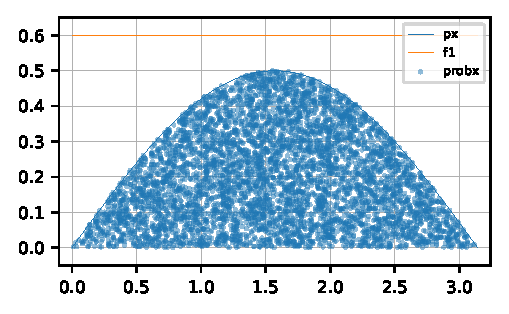
\includegraphics{CodeAndFigures/AcceptanceRejectionPlotf1.pdf}
    \caption{$f(x)=0.6$}
    \label{subfig:constant}
  \end{subfigure}
  \begin{subfigure}[b]{0.5\textwidth}
    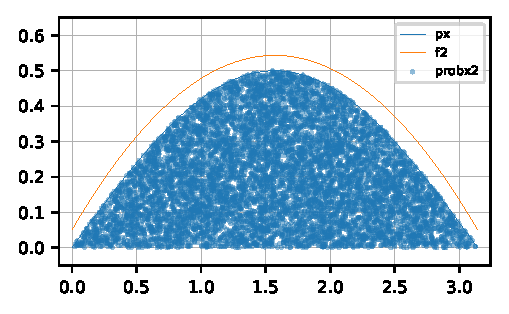
\includegraphics{CodeAndFigures/AcceptanceRejectionPlotf2.pdf}
    \caption{$f(x)=-.2x^2+.2x+.01$.}
    \label{subfig:Quadratic}
  \end{subfigure}
  \caption{Plot of random deviates from a normalized sine function using the Acceptance/Rejection Method with \ref{subfig:Quadratic} quadratic function and \ref{subfig:constant} constant function.}
  \label{fig:accRejPlot}
\end{figure}
